\clearpage
\section{nonlinear system}
The python code solving this with documentation is attached as several python files, which will be explained fully in a section of this answer. For all the tests I used the reduced chi-square test.
\subsection{Explanation of the code}

\subsection{Representative measurements}
The results from running the code for the representative measurements are 
\begin{table}[H]
    \centering 
    \begin{tabular}{c|ccc}
        Model & \(\chi^2\) & Reduced \(\chi^2\) & p-value\\
        \hline
        \(Y_1\) & 84.6 & 6.5 & \num{1.5e-12}\\
        \(Y_2\) & 163.6 & 12.6 & \num{3.7e-28}\\
        \(Y_3\) & 26.0 & 2.0 & \num{0.017}
    \end{tabular}
    \caption{The chi-square, reduced chi-square, and p-value for the best fit for each model to the representative measurement dataset.}
\end{table}
with the optimal parameters being 
\begin{table}[H]
    \centering
    \begin{tabular}{c|cccc}
        Model & A & B & C & D\\
        \hline
        \(Y_1\) & 128.56 & 0.22 & -186.57 & -133.43\\
        \(Y_2\) & -175.27 & Inf. & 0.4683 & -67.60\\
        \(Y_3\) & -1.5 & 28.04 & -100.47 & -159.35
    \end{tabular}
    \caption{Optimal parameters found using the python code. Note the infinity for B in model \(Y_2\), which results in the optimizer going to arbitrarily large values, when it's allowed to.}
\end{table}
The benefits of each hypothesis is as follows:
\begin{description}
    \item[\(Y_1\)] a sum of two sine functions with double the frequency. From plotting the representative data, it indeed looks like the data might be some kind of oscillatory behavior, so the choice makes sense. If we expect the signal to be a sine wave with sine-like disturbances, this would capture it.
    \item[\(Y_2\)] a decaying sine. The benefit of this is that it allows the ability to capture a signal whose amplitude decays over time. The problem is that if the system does not decay, this will be unable to capture the behavior.
    \item[\(Y_3\)] a cubic polynomial. The benefits are that this is a much easier hypothesis to use for calculations and to test, and it fits the dataset in this part very well. The problem is that it assumes the behavior is of a cubic equation, which relies very strongly on an assumption the data will conform to that assumption beyond the measurements in the data.
\end{description}
The initial conclusion we can reach from this data is that models \(Y_1\) and \(Y_2\) can be ruled out for this dataset. Their high reduced chi-square combined with a miniscule p-value mean that the difference between the measurements and the model's prediction are both large and highly unlikely to be statistical errors. \(Y_3\) also has a fairly high chi-square at 2 meaning the fit is still not great, but it's within workable limits.
\subsection{Real Measurement}
After looking at the raw data in a plot, I noticed that it can be broken up into two zones:
\begin{enumerate}
    \item A background measurement
    \item The signal region
\end{enumerate}
and it appears that the noise in both regions is different. The signal measurement therefore itself introduces noise which we can't account for just with the background section. Looking at a histogram of the values in the background measurement I saw it looked fairly gaussian so I ran a chi-square test which resulted in 
\begin{equation}
    \chi^2/dof=2.15, \qquad p-value=0.018
\end{equation}

which is not a great result, but given I have no other information to work off of I'll accept an assumption the noise is gaussian in the background measurement with the following parameters. A further analysis that could be made is whether the noise is somehow self-correlated, i.e that not all measurements in the noise really are random, which if removed could be characterized better by a gaussian, but this is out of scope.
\begin{align}
    \mu=-2.688\pm0.132,\qquad \sigma=3.68
\end{align}
\begin{figure}[H]
    \centering
    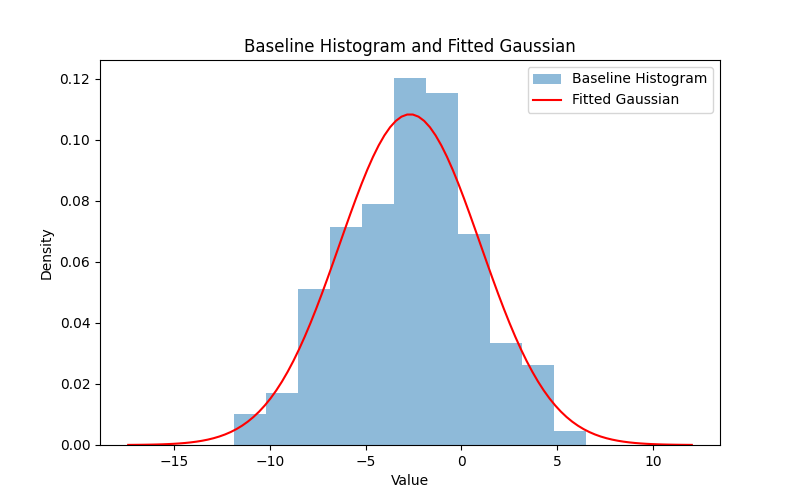
\includegraphics[width=0.75\textwidth]{noise_before_signal.png}
    \caption{Histogram of the values recorded in the section before the signal begins. A gaussian curve fit is presented on top.}
\end{figure}
To analyze the noise in the signal region, I have to first isolate the signal. Since I don't know which of the hypothesis are correct and I don't want to rush to the next part, I isolated it by performing a rolling average of the values, with a window of 20 measurements. This window was significantly smaller than the oscillations in the signal so it did not skew the signal too much. 
\begin{figure}[H]
    \centering
    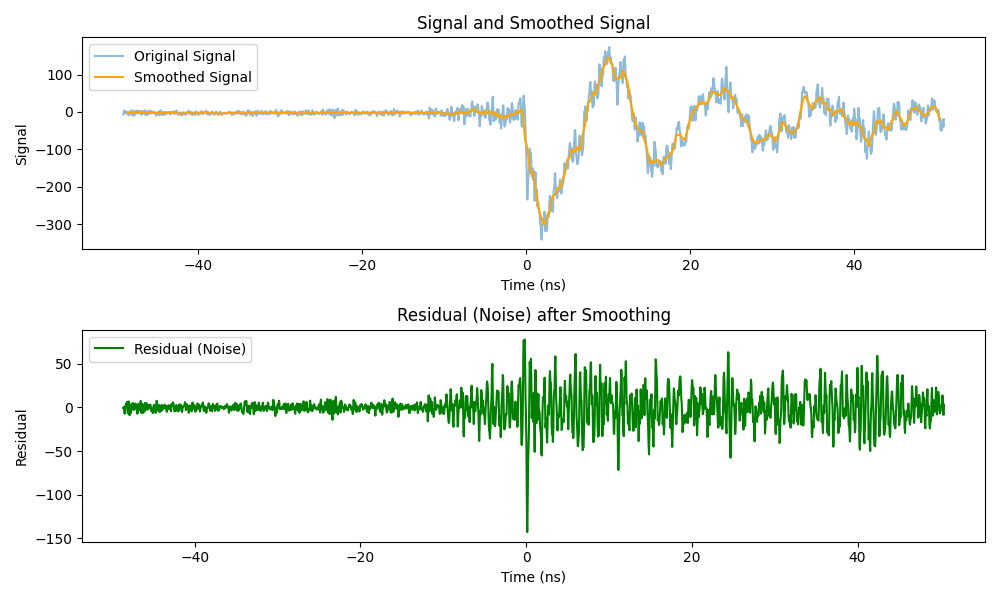
\includegraphics[width=1\textwidth]{signal_and_smoothed.png}
    \caption{Top panel: The raw data in blue and the smoothed out signal in yellow. Bottom panel: The residual, i.e the raw data with the smoothed out signal subtracted.}
\end{figure}
I then subtracted the cleaned signal from the raw data and found the noise in the signal region. After plotting a histogram of it, it also appeared quite gaussian, so I ran another chi-square test:
\begin{equation}
    \chi^2/dof=0.81, \qquad p-value=0.615
\end{equation}
which indicates that this time the noise is actually somewhat well described as gaussian:
\begin{equation}
    \mu=-0.277,\qquad \sigma=22.438
\end{equation}
\begin{figure}[H]
    \centering
    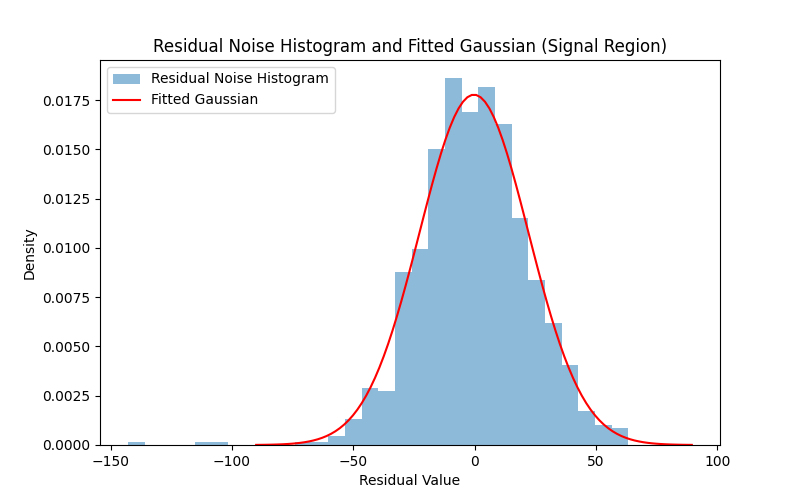
\includegraphics[width=0.75\textwidth]{noise_in_signal.png}
    \caption{Histogram of the values of the residual noise with a fitted gaussian.}
\end{figure}
next to characterize the signal I split the signal into bins of \(0.5\unit{\nano\second}\), and for each of those I calculated the mean, which is the total count \(N\), then from it subtracted the baseline noise's mean which acts as \(B\), giving me \(S=N-B\). I then calculated the error from its own standard deviation divided by the number of counts in the bin combined with the errro on \(B\).
\begin{equation}
    S_{\min}=-295\pm7\quad\text{at } t=2.11\unit{ns},\qquad S_{\max}=154\pm4\quad\text{at } t=10.11\unit{ns}
\end{equation}
with significance 
\begin{equation}
    seg_{\min}=42,\qquad seg_{\max}=36
\end{equation}
meaning the signal is highly significant in comparison to the noise.
\begin{figure}[H]
    \centering
    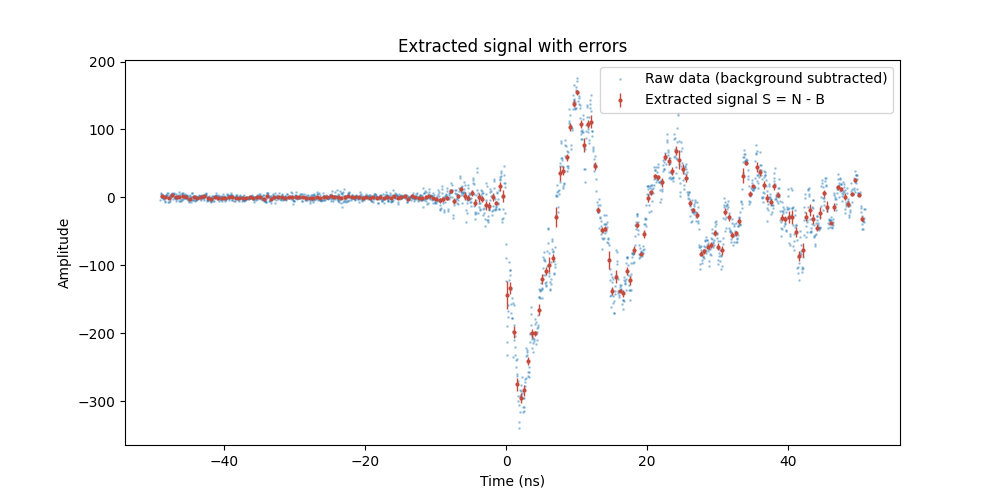
\includegraphics[width=0.75\textwidth]{extracted_signal.png}
    \caption{The raw data in blue with the extracted signal, with errorbars, on top in red.}
\end{figure}
\subsection{Simulation}
In this part all that's needed is to load and properly process the data of the simulation then run the same tests as I did for the other three hypothesis. A note on the data processing, the simulation's times are different from the others, so the times needed to be shifted. Instead of trying to manually find the right shift, I found the correct shift with the same optimization technique used for the other parameters in the question, with minimizing the chi-square between the simulation and the measured data. I decided to re-fit the hypothesis \(Y_i\) to the real measurement data from part b, to give each hypothesis its best shot. This resulted in the follwoing
\begin{table}[H]
    \centering
    \begin{tabular}{c|cc}
        Hypothesis & \(\chi^2/dof\)\\
        \hline
        \(Y_1\) & 89.98\\
        \(Y_2\) & 27.92\\
        \(Y_3\) & 221.20\\
        Simulation & 118.03
    \end{tabular}
    \caption{The reduced chi squared for each hypothesis. The p value is not presented because it is so small it underflows the precision of floating point numbers, meaning it's basically 0 for ever fit.}
\end{table}
Since the p value is effectively 0 for all of the fits, but none of the reduced chi-square tests give a good result, every hypothesis is rejected as a \emph{good} fit. But, since we were asked for the best, rather than what's good, the best fit is the one with the lowest chi-squared, that being \(Y_2\). \(Y_3\) is completely rejected because it can't capture the behavior of the data at all, and \(Y_1\) is rejected because it's simply worse. The simulation too is rejected for this reason.